\chapter{Exercise 00}
\extitle{Polynomial models II}
%%******************************************************************************%
%                                                                              %
%                                 Interlude                                    %
%                         for Machine Learning module                          %
%                                                                              %
%******************************************************************************%

% =============================== %
\section*{Interlude}
% =============================== %
\subsection*{Classification: The Art of Labelling Things}
% ******************************* %
Over the last three modules you have implemented your first machine learning algorithm.\\
\\
You are now familiar the three-steps cycle we follow when we build \textbf{learning algorithms}:
\\
\begin{figure}[!h]
    \centering
    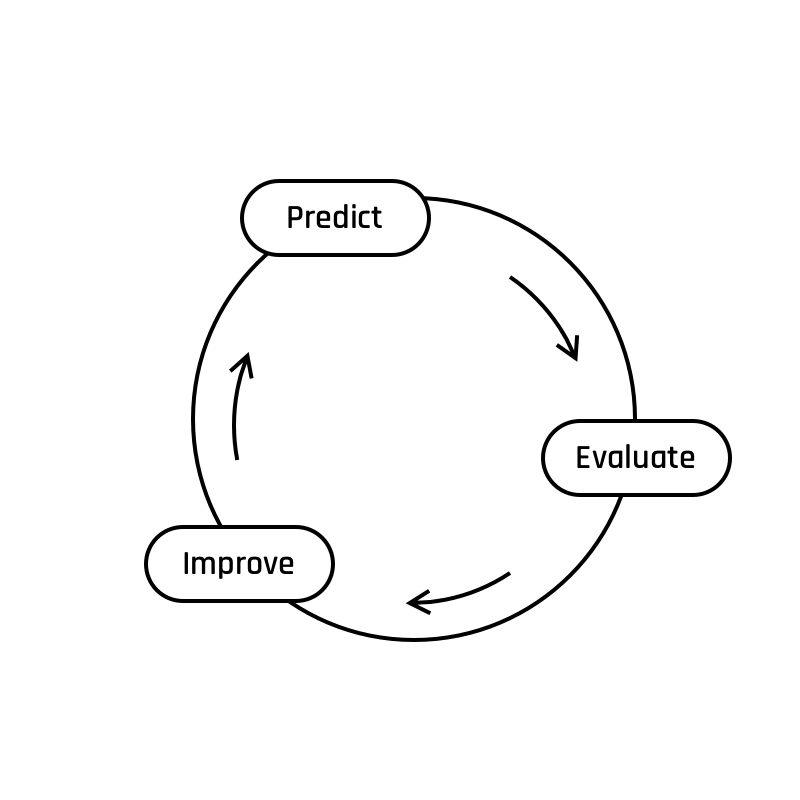
\includegraphics[scale=0.25]{assets/Default.png}
    %\caption{The Learning Cycle}
\end{figure}
\\
The first algorithm you discovered, \textbf{Multivariate Linear Regression}, can now be used to predict a numerical value, based on several features.
This algorithm uses gradient descent to optimize its loss function.\\
\\
Now let's introduce your first \textbf{classification algorithm}: the notorious \textbf{Logistic Regression.}
\hint{regression vs classification; discrete vs continuous values}
\newpage
\noindent{\textbf{Logistic regression} performs a \textit{classification task}, which means that you are not predicting a numerical value (like price, age, grades...) 
but \textbf{categories}, or \textbf{labels} (like dog, cat, sick/healty...)}.
\\
\warn{
    Don't be confused by the word \textit{'regression'} in \textbf{Logistic Regression}.
    It really is a \textit{classification task}! The name is a bit tricky but you will quickly get used to it.
    Once again: \textbf{Logistic Regression is a classification algorithm} which assigns a label/category/class to a given example.
}
\info{
    In this module we will use the following terms interchangeably: \textbf{class}, \textbf{category}, and \textbf{label}.
    They all refer to the \textit{groups} to which each training example can be assigned to, in a classification task.
}

% =============================== %
\subsection*{Predict I: Introducing the Sigmoid Function}
% ******************************* %

\begin{figure}[!h]
    \centering
    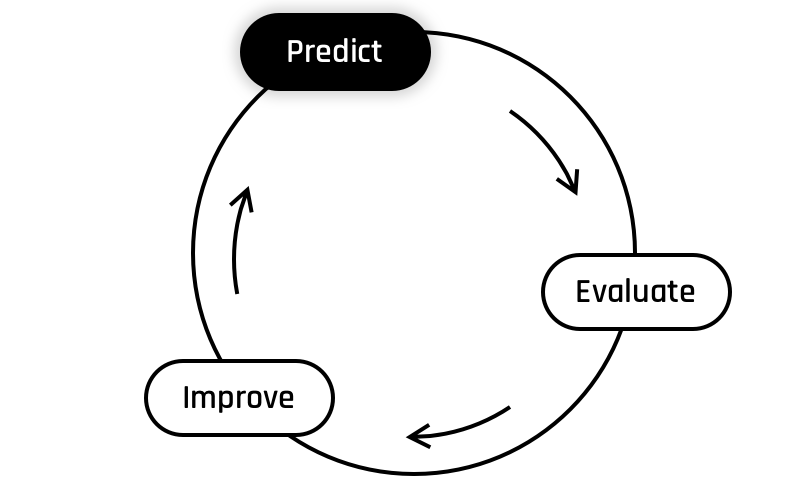
\includegraphics[scale=0.25]{assets/Predict.png}
    %\caption{The Learning Cycle - Predict}
\end{figure}

% =============================== %
\subsubsection*{Formulating a Hypothesis}
% ******************************* %
Remember that a hypothesis, denoted $h(\theta)$, is an equation that combines a set of \textbf{features} (that characterizes an example) with \textbf{parameters} in order to output a \textbf{prediction}.\\
\\
Remember the hypothesis we used in linear regression?\\
$$
h(\theta) = \theta_0 + \theta_{1} x_{1}^{(i)} + \dots + \theta_{n} x_{n}^{(i)} = \theta \cdot x'^{(i)}
$$
\newline
It worked fine to predict continuous values, but could we also use it to tell, for example, 
if a patient is sick or not?
That's a yes-or-no question, so the output from the hypothesis function should reflect that.\\
\\
To get started, we will assign each class a numerical value: sick patients will be 
assigned a value of 1, and healthy patients will be assigned a value of 0.\\
The goal will be to build a hypothesis that outputs a probability that a patient is sick as a float number in the range of [0, 1].\\
\\
The good news is that we can keep the linear equation we already worked with!\\
\\
All we need to do is squash its output through another function that is bounded between 0 and 1.\\
\\
That's the purpose of the \textbf{Sigmoid function} and your next assignment is to implement it!

%\newpage
\turnindir{ex00}
\exnumber{00}
\exfiles{polynomial\_model\_extended.py}
\exforbidden{sklearn}
\makeheaderfilesforbidden

% ================================== %
\section*{Objective}
% ---------------------------------- %
Create a function that takes a matrix $X$ of dimensions $(m \times n)$ and an integer $p$ as input, and returns a matrix of dimension $(m \times (np))$.
For each column $x_j$ of the matrix $X$, the new matrix contains
$x_j$ raised to the power of $k$, for $k = 1, 2, ..., p$ :

$$
x_1  \mid  \ldots  \mid  x_n  \mid  x_1^2  \mid  \ldots  \mid  x_n^2  \mid  \ldots  \mid  x_1^p  \mid  \ldots  \mid  x_n^p
$$

% ================================== %
\section*{Instructions}
% ---------------------------------- %
In the \texttt{polynomial\_model\_extended.py} file, write the following function as per the instructions given below:

\begin{minted}[bgcolor=darcula-back,formatcom=\color{lightgrey},fontsize=\scriptsize]{python}
def add_polynomial_features(x, power):
	"""Add polynomial features to matrix x by raising its columns to every power in the range of 1 up to the power given in argument.  
	Args:
		x: has to be an numpy.ndarray, a matrix of shape m * n.
		power: has to be an int, the power up to which the columns of matrix x are going to be raised.
	Returns:
		The matrix of polynomial features as a numpy.ndarray, of shape m * (np), containg the polynomial feature values for all training examples.
		None if x is an empty numpy.ndarray.
	Raises:
		This function should not raise any Exception.
	"""
	... Your code ...
\end{minted}


% ================================== %
\section*{Examples}
% ---------------------------------- %

\begin{minted}[bgcolor=darcula-back,formatcom=\color{lightgrey},fontsize=\scriptsize]{python}
import numpy as np
x = np.arange(1,11).reshape(5, 2)

# Example 1:
add_polynomial_features(x, 3)
# Output:
array([[   1,    2,    1,    4,    1,    8],
       [   3,    4,    9,   16,   27,   64],
       [   5,    6,   25,   36,  125,  216],
       [   7,    8,   49,   64,  343,  512],
       [   9,   10,   81,  100,  729, 1000]])

# Example 2:
add_polynomial_features(x, 4)
# Output:
array([[    1,     2,     1,     4,     1,     8,     1,    16],
       [    3,     4,     9,    16,    27,    64,    81,   256],
       [    5,     6,    25,    36,   125,   216,   625,  1296],
       [    7,     8,    49,    64,   343,   512,  2401,  4096],
       [    9,    10,    81,   100,   729,  1000,  6561, 10000]])
\end{minted}